\icode{E-MD-CA-L3-261112-011}
如图所示，质量 \(M =\) \,\qty{1}{kg}、长度 \(L =\) \,\qty{1}{m}的木板 \(A\) 静止在水平面上，\(A\) 与水平面间的动摩擦因数 \(\mu_1 = 0.1\)。在 \(A\) 的左端放置一质量 \(m =\) \,\qty{1}{kg}的铁块 \(B\)（可视为质点），\(B\) 与 \(A\) 间的动摩擦因数 \(\mu_2 = 0.3\)，现用一水平恒力 \(F\) 作用在 \(B\) 上，取 \(g =\) \,\qty{10}{m/s^2}，设滑动摩擦力等于最大静摩擦力。求：
\begin{enumerate}
	\item 要保持 \(A\)、\(B\) 一起做匀加速运动，求力 \(F\) 的取值范围；
	\item 若 \(F =\) \,\qty{5}{N}，求铁块运动到木块右端所用的时间。
\end{enumerate}

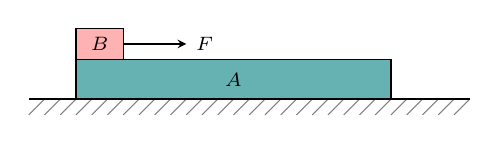
\begin{tikzpicture}[>=stealth,font=\scriptsize]
	\draw[fill=teal!60] (0,0) rectangle(4,.5)node[midway]{\(A\)};
	\draw[fill=red!30] (0,.5) rectangle(.6,.9)node[midway]{\(B\)};
	\draw[->] (.6,.7)--++(.8,0)node[right]{\(F\)};
	\foreach \x in {-.6,-.4,...,5}
		\draw[gray] (\x,-.2)--++(.2,.2);
	\draw[thick] (-.6,0)--(5,0);
\end{tikzpicture}
\begin{answer}
	（1）\(2 < F \leq 4\) \qty{}{N}（2）\(\sqrt{2}\)\qty{}{s}
\end{answer}